% Options for packages loaded elsewhere
\PassOptionsToPackage{unicode}{hyperref}
\PassOptionsToPackage{hyphens}{url}
%
\documentclass[
]{book}
\usepackage{lmodern}
\usepackage{amsmath}
\usepackage{ifxetex,ifluatex}
\ifnum 0\ifxetex 1\fi\ifluatex 1\fi=0 % if pdftex
  \usepackage[T1]{fontenc}
  \usepackage[utf8]{inputenc}
  \usepackage{textcomp} % provide euro and other symbols
  \usepackage{amssymb}
\else % if luatex or xetex
  \usepackage{unicode-math}
  \defaultfontfeatures{Scale=MatchLowercase}
  \defaultfontfeatures[\rmfamily]{Ligatures=TeX,Scale=1}
\fi
% Use upquote if available, for straight quotes in verbatim environments
\IfFileExists{upquote.sty}{\usepackage{upquote}}{}
\IfFileExists{microtype.sty}{% use microtype if available
  \usepackage[]{microtype}
  \UseMicrotypeSet[protrusion]{basicmath} % disable protrusion for tt fonts
}{}
\makeatletter
\@ifundefined{KOMAClassName}{% if non-KOMA class
  \IfFileExists{parskip.sty}{%
    \usepackage{parskip}
  }{% else
    \setlength{\parindent}{0pt}
    \setlength{\parskip}{6pt plus 2pt minus 1pt}}
}{% if KOMA class
  \KOMAoptions{parskip=half}}
\makeatother
\usepackage{xcolor}
\IfFileExists{xurl.sty}{\usepackage{xurl}}{} % add URL line breaks if available
\IfFileExists{bookmark.sty}{\usepackage{bookmark}}{\usepackage{hyperref}}
\hypersetup{
  pdftitle={Bygge statistisk modeller med kategoriske variabler (ANOVA, t-test)},
  pdfauthor={Christian Magelssen},
  hidelinks,
  pdfcreator={LaTeX via pandoc}}
\urlstyle{same} % disable monospaced font for URLs
\usepackage{color}
\usepackage{fancyvrb}
\newcommand{\VerbBar}{|}
\newcommand{\VERB}{\Verb[commandchars=\\\{\}]}
\DefineVerbatimEnvironment{Highlighting}{Verbatim}{commandchars=\\\{\}}
% Add ',fontsize=\small' for more characters per line
\usepackage{framed}
\definecolor{shadecolor}{RGB}{248,248,248}
\newenvironment{Shaded}{\begin{snugshade}}{\end{snugshade}}
\newcommand{\AlertTok}[1]{\textcolor[rgb]{0.94,0.16,0.16}{#1}}
\newcommand{\AnnotationTok}[1]{\textcolor[rgb]{0.56,0.35,0.01}{\textbf{\textit{#1}}}}
\newcommand{\AttributeTok}[1]{\textcolor[rgb]{0.77,0.63,0.00}{#1}}
\newcommand{\BaseNTok}[1]{\textcolor[rgb]{0.00,0.00,0.81}{#1}}
\newcommand{\BuiltInTok}[1]{#1}
\newcommand{\CharTok}[1]{\textcolor[rgb]{0.31,0.60,0.02}{#1}}
\newcommand{\CommentTok}[1]{\textcolor[rgb]{0.56,0.35,0.01}{\textit{#1}}}
\newcommand{\CommentVarTok}[1]{\textcolor[rgb]{0.56,0.35,0.01}{\textbf{\textit{#1}}}}
\newcommand{\ConstantTok}[1]{\textcolor[rgb]{0.00,0.00,0.00}{#1}}
\newcommand{\ControlFlowTok}[1]{\textcolor[rgb]{0.13,0.29,0.53}{\textbf{#1}}}
\newcommand{\DataTypeTok}[1]{\textcolor[rgb]{0.13,0.29,0.53}{#1}}
\newcommand{\DecValTok}[1]{\textcolor[rgb]{0.00,0.00,0.81}{#1}}
\newcommand{\DocumentationTok}[1]{\textcolor[rgb]{0.56,0.35,0.01}{\textbf{\textit{#1}}}}
\newcommand{\ErrorTok}[1]{\textcolor[rgb]{0.64,0.00,0.00}{\textbf{#1}}}
\newcommand{\ExtensionTok}[1]{#1}
\newcommand{\FloatTok}[1]{\textcolor[rgb]{0.00,0.00,0.81}{#1}}
\newcommand{\FunctionTok}[1]{\textcolor[rgb]{0.00,0.00,0.00}{#1}}
\newcommand{\ImportTok}[1]{#1}
\newcommand{\InformationTok}[1]{\textcolor[rgb]{0.56,0.35,0.01}{\textbf{\textit{#1}}}}
\newcommand{\KeywordTok}[1]{\textcolor[rgb]{0.13,0.29,0.53}{\textbf{#1}}}
\newcommand{\NormalTok}[1]{#1}
\newcommand{\OperatorTok}[1]{\textcolor[rgb]{0.81,0.36,0.00}{\textbf{#1}}}
\newcommand{\OtherTok}[1]{\textcolor[rgb]{0.56,0.35,0.01}{#1}}
\newcommand{\PreprocessorTok}[1]{\textcolor[rgb]{0.56,0.35,0.01}{\textit{#1}}}
\newcommand{\RegionMarkerTok}[1]{#1}
\newcommand{\SpecialCharTok}[1]{\textcolor[rgb]{0.00,0.00,0.00}{#1}}
\newcommand{\SpecialStringTok}[1]{\textcolor[rgb]{0.31,0.60,0.02}{#1}}
\newcommand{\StringTok}[1]{\textcolor[rgb]{0.31,0.60,0.02}{#1}}
\newcommand{\VariableTok}[1]{\textcolor[rgb]{0.00,0.00,0.00}{#1}}
\newcommand{\VerbatimStringTok}[1]{\textcolor[rgb]{0.31,0.60,0.02}{#1}}
\newcommand{\WarningTok}[1]{\textcolor[rgb]{0.56,0.35,0.01}{\textbf{\textit{#1}}}}
\usepackage{longtable,booktabs}
\usepackage{calc} % for calculating minipage widths
% Correct order of tables after \paragraph or \subparagraph
\usepackage{etoolbox}
\makeatletter
\patchcmd\longtable{\par}{\if@noskipsec\mbox{}\fi\par}{}{}
\makeatother
% Allow footnotes in longtable head/foot
\IfFileExists{footnotehyper.sty}{\usepackage{footnotehyper}}{\usepackage{footnote}}
\makesavenoteenv{longtable}
\usepackage{graphicx}
\makeatletter
\def\maxwidth{\ifdim\Gin@nat@width>\linewidth\linewidth\else\Gin@nat@width\fi}
\def\maxheight{\ifdim\Gin@nat@height>\textheight\textheight\else\Gin@nat@height\fi}
\makeatother
% Scale images if necessary, so that they will not overflow the page
% margins by default, and it is still possible to overwrite the defaults
% using explicit options in \includegraphics[width, height, ...]{}
\setkeys{Gin}{width=\maxwidth,height=\maxheight,keepaspectratio}
% Set default figure placement to htbp
\makeatletter
\def\fps@figure{htbp}
\makeatother
\setlength{\emergencystretch}{3em} % prevent overfull lines
\providecommand{\tightlist}{%
  \setlength{\itemsep}{0pt}\setlength{\parskip}{0pt}}
\setcounter{secnumdepth}{5}
\usepackage{booktabs}

\newenvironment{danger}
    {
    \hline\\
    }
    { 
    \\\\\hline
    }
    
\newenvironment{warning}
    {
    \hline\\
    }
    { 
    \\\\\hline
    }
    
\newenvironment{info}
    {
    \hline\\
    }
    { 
    \\\\\hline
    }
    
\newenvironment{try}
    {
    \hline\\
    }
    { 
    \\\\\hline
    }
\ifluatex
  \usepackage{selnolig}  % disable illegal ligatures
\fi
\usepackage[]{natbib}
\bibliographystyle{apalike}

\title{Bygge statistisk modeller med kategoriske variabler (ANOVA, t-test)}
\author{Christian Magelssen}
\date{2021-04-03}

\begin{document}
\maketitle

{
\setcounter{tocdepth}{1}
\tableofcontents
}
\hypertarget{intro}{%
\chapter{Introduksjon}\label{intro}}

I dette kapittelet skal vi lære å bygge statistiske modeller for å teste om \textbf{to eller flere grupper er forskjellige på en avhengig variabel som er kontinuerlig}.

En variabel kan sies å være \textbf{kontinuerlig} når vi kan bestemme hvor presist vi ønsker å måle den. For eksempel regnes tid som en kontuerlig variabel fordi det (i prinsippet) ikke finnes noen grenser hvor presist vi kan måle det; vi kan måle det i år, måneder, uker, dager, timer, minutter, sekunder, tideler, hundredeler eller tusendeler.

\textbf{Grupper} defineres i psykologifaget som en samling mennesker som deler bestemte karakterstikker. Det kan være spillere på et fotballag, individer på et treningssenter, eller menn og kvinner. Dette er også eksempler på naturlig inndelte grupper i samfunnet. Noen ganger kan det være interessant å se om disse gruppene er forskjellige. For eksempel kan det være interessant å se om individer som trener på treningssenter er sterkere enn de som ikke trener på treningssenter.

Andre ganger kan det være interessant å teste om to grupper, som var like før et eksperiment, har blitt forskjellige fordi vi har behandlet dem ulikt. Vi randomiserer individer i to ulike grupper, slik at vi sikrer at vi blander disse individene godt (f.eks kjønn, motivasjon, interesser). Hvis eksperimentet har blitt gjennomført godt at det ikke er noen andre forklaringer på at disse to gruppene har blitt forskjellige etter intervensjonsperioden, så kan vi trekke en slutning om disse to gruppene trolig ikke kommer fra samme populasjon lenger; eksperimentet har gjort at disse to gruppene trolig kommer fra to forskjellige populasjoner.

\hypertarget{datasett}{%
\chapter{Datasett}\label{datasett}}

\hypertarget{buxf8r-man-trene-med-ett-eller-flere-sett-i-styrketrening}{%
\section{Bør man trene med ett eller flere sett i styrketrening?}\label{buxf8r-man-trene-med-ett-eller-flere-sett-i-styrketrening}}

Mange utrente lurer på hvor mange serier de bør gjennnomføre for å oppnå maksimal treningseffekt i styrketrening. Noen føler at de blir slitne etter ett sett og at dette derfor er tilstrekkelig. Andre mener at et hardere treningstimuli er nødvendig, selv om man er utrent, og at to eller flere sett derfor er bedre. En forsker som var tidlig ute med å undersøke var Bent Rønnestad \citep{ronnestad_dissimilar_2007}

Eksperimentet ble gjennomført som et \textbf{between-subject design} med to grupper:en gruppe trente 1 sett på underkroppen og 3 sett på overkroppen; En annen gruppe trente 3 sett på underkroppen og 1 sett på overkroppen. Disse gruppene kalte han henholdsvis \textbf{1L-3U} og \textbf{3L-1U} (L=lower; U=Upper).

De to gruppene trente 3 ganger i uken i totalt 11 uker. Forskergruppen ville så se hva som ga mest fremgang i 1RM på underkroppsøvelser. Den avhengige variabelen ble derfor \%-fremgang på 1RM på underkroppsøvelser.

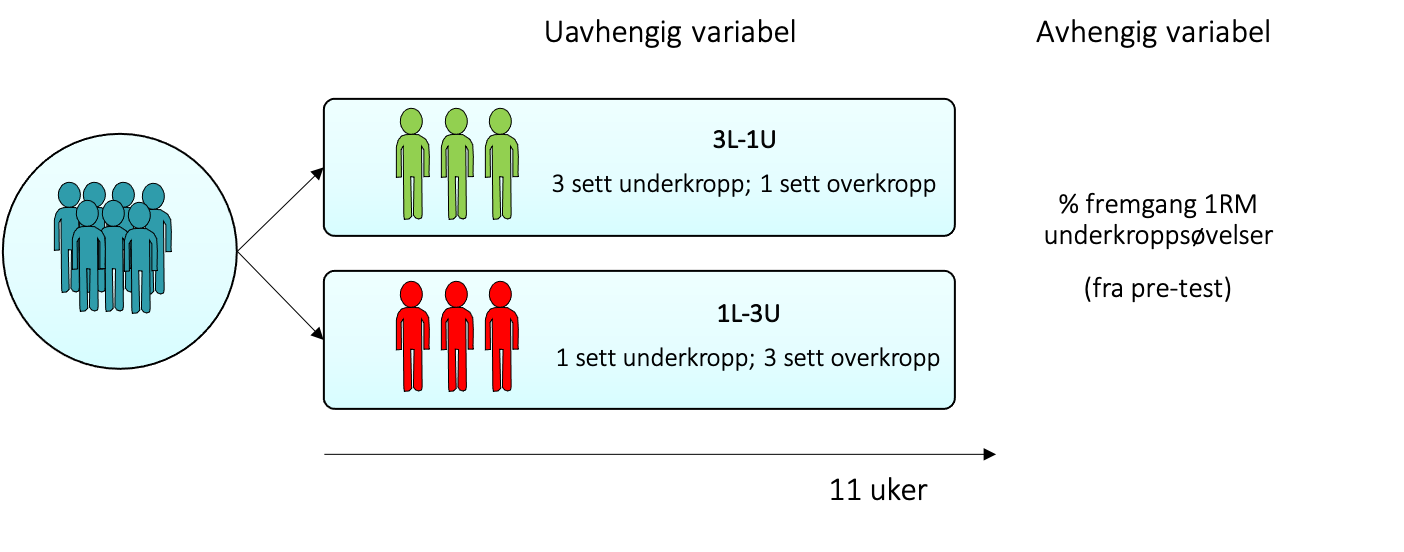
\includegraphics{design.png}
Vi har ikke tilgang til dette datasettet, men vi har simulert dette datasettet i R basert på verdiene som ble oppgitt i artikkelen. Datasettet blir tilnærmet likt, men siden det er en simulering blir det aldri helt identisk. Datasettet ser du i tabellen under.

\begin{table}

\caption{\label{tab:unnamed-chunk-3}Simulert datasett}
\centering
\begin{tabular}[t]{rlr}
\toprule
individ & gruppe & rm\\
\midrule
1 & tre.sett & 40.46704\\
2 & tre.sett & 49.07223\\
3 & tre.sett & 47.94131\\
4 & tre.sett & 44.51389\\
5 & tre.sett & 52.28750\\
\addlinespace
6 & tre.sett & 40.01750\\
7 & tre.sett & 49.48425\\
8 & tre.sett & 29.21048\\
9 & tre.sett & 40.59293\\
10 & tre.sett & 37.58676\\
\addlinespace
11 & tre.sett & 35.42651\\
12 & tre.sett & 42.49354\\
13 & ett.sett & 17.70576\\
14 & ett.sett & 17.07181\\
15 & ett.sett & 18.26811\\
\addlinespace
16 & ett.sett & 25.42594\\
17 & ett.sett & 32.70313\\
18 & ett.sett & 19.10226\\
19 & ett.sett & 22.23827\\
20 & ett.sett & 22.27148\\
\addlinespace
21 & ett.sett & 26.17889\\
22 & ett.sett & 20.34857\\
23 & ett.sett & 23.52773\\
24 & ett.sett & 17.95966\\
\bottomrule
\end{tabular}
\end{table}

Du kan få nøyaktig samme datsett ved å klippe ut og lime inn følgende kode i en skript-fil i R (husk å laste inn tidyverse-pakken, library(tidyverse) ). Du kan også laste ned datasettet som en .csv fil fra canvas.

\begin{Shaded}
\begin{Highlighting}[]
\FunctionTok{set.seed}\NormalTok{(}\DecValTok{2002}\NormalTok{) }\CommentTok{\#viktig å ha med denne for å få nøyaktig samme datasett}
\NormalTok{tre.sett }\OtherTok{\textless{}{-}} \FunctionTok{rnorm}\NormalTok{(}\AttributeTok{n =} \DecValTok{12}\NormalTok{, }\AttributeTok{mean =} \DecValTok{41}\NormalTok{, }\AttributeTok{sd =} \DecValTok{5}\NormalTok{) }\CommentTok{\#12 individer}
\NormalTok{ett.sett }\OtherTok{\textless{}{-}}\FunctionTok{rnorm}\NormalTok{(}\AttributeTok{n =} \DecValTok{12}\NormalTok{, }\AttributeTok{mean =} \DecValTok{21}\NormalTok{, }\AttributeTok{sd =} \DecValTok{5}\NormalTok{) }\CommentTok{\#12 individer}

\CommentTok{\#lager en tibble fra tidyverse{-}pakken. Må ha lastet inn tidyverse library(tidyverse) i scriptfilen}
\NormalTok{dat }\OtherTok{\textless{}{-}} \FunctionTok{tibble}\NormalTok{(}\AttributeTok{individ =} \FunctionTok{seq}\NormalTok{(}\DecValTok{1}\SpecialCharTok{:}\DecValTok{24}\NormalTok{),}
              \AttributeTok{gruppe =} \FunctionTok{rep}\NormalTok{(}\FunctionTok{c}\NormalTok{(}\StringTok{"tre.sett "}\NormalTok{, }\StringTok{"ett.sett"}\NormalTok{), }\FunctionTok{c}\NormalTok{(}\FunctionTok{length}\NormalTok{(tre.sett), }\FunctionTok{length}\NormalTok{(ett.sett))),}
              \AttributeTok{rm =} \FunctionTok{c}\NormalTok{(tre.sett , ett.sett))}
\end{Highlighting}
\end{Shaded}

\textbf{Oppgave}
Før du går videre er det greit at du gjør deg kjent med datasettet som vi har generert. Studer datasettet og svar på følgende spørsmål:

\begin{enumerate}
\def\labelenumi{\alph{enumi})}
\tightlist
\item
  Hvor mange kolonner er det i tabellen over?
\item
  Hvor mange deltakere var med i studien?
\item
  Hvilke to verdier kan variabelen gruppe? og
\end{enumerate}

\hypertarget{gjennomsnitt-for-de-to-gruppene}{%
\section{Gjennomsnitt for de to gruppene}\label{gjennomsnitt-for-de-to-gruppene}}

Bra! Det er alltid viktig å bli kjent med sitt eget datasett, men nå som du har det kan vi gå videre. Vi er interessert i om det er forskjeller mellom de to gruppene (``tre.sett'' vs.~ett.sett) på \% fremgang fra pre- til post-test. Så kanskje vi kan starte med å se om det er forskjeller i gjennomsnitt mellom to gruppene? Dette kan enkelt gjøres i R, Jamovi eller excel. Her er en kode for å gjøre dette i R:

\begin{Shaded}
\begin{Highlighting}[]
\CommentTok{\#jeg lager et oobjekt som heter mean\_rm }
\NormalTok{mean\_rm }\OtherTok{\textless{}{-}}\NormalTok{ dat }\SpecialCharTok{\%\textgreater{}\%}
  \CommentTok{\#Jeg grupperer etter gruppe, slik at jeg får et mean for hver gruppe istf. for å få mean for alle individene}
  \CommentTok{\#group\_by er en funksjon for dette}
  \FunctionTok{group\_by}\NormalTok{(gruppe) }\SpecialCharTok{\%\textgreater{}\%}
  \CommentTok{\#deretter bruker jeg summarise funksjonen for å regne gjennomsnitt}
  \FunctionTok{summarise}\NormalTok{(}\AttributeTok{mean.fremgang.1RM =} \FunctionTok{mean}\NormalTok{(rm))}
\end{Highlighting}
\end{Shaded}

Koden gir oss følgende tabell:
\textbackslash begin\{table\}

\textbackslash caption\{\label{tab:unnamed-chunk-6}Gjennomsnittlige \%-vis fremgang for de to gruppene\}
\centering

\begin{tabular}[t]{lr}
\toprule
gruppe & mean.fremgang.1RM\\
\midrule
ett.sett & 21.90013\\
tre.sett & 42.42450\\
\bottomrule
\end{tabular}

\textbackslash end\{table\}
\textbf{Oppgave}
a) Hvilken gruppe hadde mest fremgang?
ett.sett tre.sett`

\hypertarget{figur-av-datasettet}{%
\section{Figur av datasettet}\label{figur-av-datasettet}}

Vi kan også presentere dataen i en figur. For denne typen data er det veldig vanlig å bruke et \textbf{stolpediagram}:

\begin{figure}

{\centering 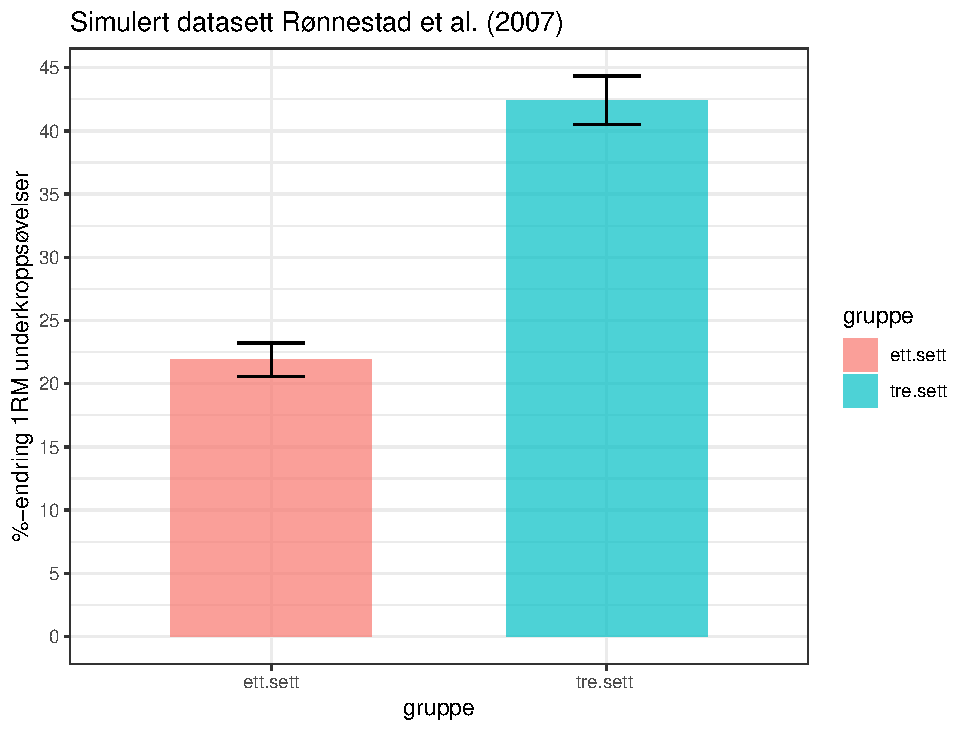
\includegraphics[width=0.8\linewidth]{02-datasett_files/figure-latex/nice-fig-1} 

}

\caption{Here is a nice figure!}\label{fig:nice-fig}
\end{figure}

Et stolpediagram er pent å se på, men er egentlig designet for å kategoriske data. For eksempel er det fint å bruke dette når vi skal presentere frekvensen antall som har kjørt bil til skolen og antall personer som har gått. Les \citep{weissgerber_beyond_2015}(\url{https://journals.plos.org/plosbiology/article?id=10.1371/journal.pbio.1002128}). Deretter svar på følgende spørsmål for å se om du har forstått problemene ved å bruke stolpediagram på kontinuerlig data.

\textbf{Oppgave}.

\begin{enumerate}
\def\labelenumi{\alph{enumi}.}
\item
  Stolpediagram er designet for kontinuerlig kategorisk data.
\item
  Høyden på stolpen representerer (bruk det norske begrepet!), hvilket vil si at det også må ligge noen observasjoner over og under stolpen.
\item
  Et stolpediagram viser ikke standard error standardavvik CI fordelingen av observasjonene, og dette spesielt være problematisk ved store små.
\item
  Forfatterne av artikkelen anbefaler mer bruk av bar graph scatterplot for kontinuerlige variabler.
\item
  Ofte er det brukt error sammen med stolpediagram.
\end{enumerate}

Hvis man likevel ønsker å bruke et stolpediagram for å presentere dataen er det viktig at man forteller om man har brukt SE, SD eller CI. Stanard error for gjennomsnittet regnes ved å ta \(SD/sqrt(N)\), så ved store utvalg vil standard error være høyt lite. Standardavviket er kun \(sqrt(varians/n-1)\), så denne vil i større mindre grad være påvirket av utvalgsstørrelsen".

\hypertarget{koding-av-kategoriske-variabler}{%
\chapter{Koding av kategoriske variabler}\label{koding-av-kategoriske-variabler}}

I tabellen på s. kan du se at vi har en tabell med tre kolonner: en kolonne for hver variabel vi har i vårt datasett. Variabelen \textbf{gruppe} er en kategorisk vaiabel som har to ulike verdier: ``ett.sett'' og ``tre.sett''. Dette er de to gruppene som vi skal teste om er forskjellige. I programmeringsverdenen kalles disse denne typen data for et tekstobjekt, ``strings'' (python/javascript) eller ``characters'' (R). På norsk kalles disse verdiene for ord. Uansett navn er problemet at vi ikke kan putte ord inn i en statistisk modell; vi er nødt til å representere denne kategoriske vaiabelen med tallverdier. Det er flere måter å gjøre dette på, men de forskjellige måtene gir ulik resultat. Derfor må vi vie en god del tid på dette. Vi går gjennom to måter å gjøre dette på.

\hypertarget{dummykoding}{%
\section{Dummykoding}\label{dummykoding}}

En vanlig metode kalles \textbf{dummykoding} eller \textbf{treatment-koding}. Den går ut på å lage en eller flere variabler med 0 og 1 som de to mulige verdiene. Antall variabler vi trenger avhenger av antall grupper vi vil sammenligne. Siden vårt datasett kun inneholder to grupper, så trenger vi kun en variabel. Vi kan den ene gruppen og den andre 1. Hovedregelen er at vi gir 0 til baselinegruppe og 1 til den eksperimentelle gruppen. Vi gir derfor 0 til 1.sett-gruppen og 1 til 3.sett-gruppen. Gjør dette før du går videre.

I R og Jamovi kan du gjøre det med følgende if/else statement. I R kan du bruke følgende kode:

\begin{Shaded}
\begin{Highlighting}[]
\CommentTok{\#lager et nytt objekt som heter dummykodet.dat}
\NormalTok{dummykodet.dat }\OtherTok{\textless{}{-}}\NormalTok{ dat }\SpecialCharTok{\%\textgreater{}\%}
  \CommentTok{\# her lager jeg en ny kolonne som heter dummykoder. If gruppe == \textquotesingle{}ett.sett\textquotesingle{}, gi verdien 0, else gi de 1.}
  \FunctionTok{mutate}\NormalTok{(}\AttributeTok{dummykodet =} \FunctionTok{if\_else}\NormalTok{(gruppe }\SpecialCharTok{==} \StringTok{"ett.sett"}\NormalTok{, }\DecValTok{0}\NormalTok{, }\DecValTok{1}\NormalTok{))}
\end{Highlighting}
\end{Shaded}

I jamovi ville jeg sett følgende video:

\hypertarget{bygge-statistisk-modeller}{%
\chapter{Bygge statistisk modeller}\label{bygge-statistisk-modeller}}

\hypertarget{hensikten-med-modellbygging}{%
\section{Hensikten med modellbygging}\label{hensikten-med-modellbygging}}

Straks forskere har samlet inn dataen de trenger er den neste oppgave å bygge statistsike modeller som beskriver denne dataen. Hvis en modell er god, kan vi predikere hva en person har skåret på utfallsvariablen uten å bomme altfor mye. Hvis en modell er dårlig bør vi ikke bruke den. I vårt tilfelle ønsker vi å bygge modeller som sier noe om hva en person hadde i \% fremgang i 1RM maks.

Modellene vi skal bygge vil alltid være en variant av ligningen under. Vi bare bytter ut det i parantesen med en spesifikk modell som vi ønsker å bygge.

\[
data_i = (modell) + error_i
\]

Mange frykter ligninger. Vi også. Men det er ikke så ille når man blir vant til det, og det kommer vi til å bli med litt øving. Som vi sa kommer vi til å bruke denne ligningen til alle være statistiske tester. Dessuten hjelper ligninger oss til å huske informasjon bedre

La oss bryte denne ligningen ned:

\textbf{Data} er den faktiske observasjonen et individ har hatt på den avhengige variablen. I dette tilfellet er det fremgang i 1RM underkropp. Legg merke til den lille i -en som står bak data og error i ligningen. Denne betyr individ og betyr bare at vi kan bruke en modell til å si noe om hva at individ hadde på den avhengig variabelen. Vi kan erstatte i -en med 3 eller 8. Da betyr det bare at vi kan bruke en modell til å si noe om individ 3 og 8. Vi bruker i for å holde det generelt. Statistikere bruker ofte begrepet begrepet predikere. Å predikere er et verb synonymt med å forutsi. Min måte å tenke på det er at vi ønsker å si hva en person hadde som faktisk observasjon på den målte avhengig variabelen.

\textbf{Modell} er egentlig bare en representasjon av denne dataen, mens \textbf{error} er hvor mye modellen bommer fra den faktisk observasjonen (dvs. data). Dette blir nok mer oppklarende om vi bruker et eksempel:

Forestill deg at du er lege, og at du får inn en pasient som sier hun har feber. Du vet at den normale kroppstemperaturen er 37, så da kan vi bruke 37 som modell.

\[
kroppstemperatur_i = 37 + error_i
\]
Det neste du gjør er å ta en febermåling av pasienten, og du måler kroppstemperaturen hennes til å være 40.

\[
40 = 37 + error
\]
Modellen din tar feil med 3 grader, fordi 40-37 = 3. Vi kaller slike feil for error.

\[
40 = 37 + 3
\]
Formelt sett regner vi error for en hvilken som helst modell ved å få error i ligningen alene, ved å reorganisere ligningen.

\[
data_i = modell + error_i
\]
\[
error_i = data_i - modell
\]
\[
3 = 40 - 37
\]
Gratulerer, du har bygget din første modell. Denne modellen var riktignok nokså enkel, men du vil nok se at det vi skal gjøre videre ikke er så annerledes. Vi bygger riktignok ikke modeller for å passe perfekt til ett enkelt individ, men til et helt datasett. I en studie har du ofte mange deltakere med, og modellen vi skal bygge bør være en god representasjon av disse individene. Med andre ord bør erroren i modell være så liten som mulig. \textbf{Dette er viktig!} Vi ønsker å bygge statistiske modeller som er gode, og vi ønsker å sammenligne ulike modeller for å se hvilke av disse modellene som reduserer erroren mest mulig.

Det er en mer korrekt og presis måte å skrive ligningen under på, og som du ofte ser i artikler og statistikkbøker:

\begin{quote}
\begin{quote}
Vi kommer til å benytte denne måten å skrive på fordi det er den dere ser i statistikkbøker og artikler. Tolkningen er akkurat lik.
\end{quote}
\end{quote}

\[
data_i = (modell) + error_i
\]
\[
Y_i = (b_0) + error_i
\]
Her er \(Y_i\) den avhengige variabelen som vi faktisk har målt for et individ, \emph{i}. Hvis det kun står \(b_0\), så betyr det at vi kun estimerer ett enkelt parameter. I slike tilfeller bruker vi kun ett enkelt parameter til å si noe om hva det enkelte individ hadde i observasjon på den avhengig variabelen, og da predikerer modellen likt for alle individene.

Vi kan også bruke en mer kompleks modell, som i ligningen under:

\[
Y_i = (b_0 + b_1X_i) + error
\]
\textbf{X\_i} er dette individets faktiske måling på variabel, X, som vi ofte kaller for prediktorvariabel. Prediktorvariabelen har også \(b_1\) hektet på seg. Denne forteller oss forholdet mellom prediktorvariabelen (Xi) og den avhengig variabelen (Yi). b\_0 blir her vår prediksjon når Xi er \textbf{null} og \textbf{0}.

\begin{quote}
\begin{quote}
Figuren under gjør ligningen i mer forståelig
\end{quote}
\end{quote}

I figurene under ser tre ulike modeller med uinteressante X og Y variabler. Alle har samme b0, mens de har forskjellig b1. Husk at b1 forteller om forholdet mellom X og Y. I \textbf{modell A} ser du at når X øker så øker Y med 0.4 \textbf{for hver enhets økning i X}.

\begin{quote}
\begin{quote}
Dette er slik du skal tolke b1. For hver enhets økning i X, dvs gå fra 1 til 2, så forventer vi at Y øker med. På norsk kalles b1 for stigningstallet
\end{quote}
\end{quote}

I \textbf{modell B} er det ingen relasjon mellom X og Y, så for en enhets økning i X, vil vi forvente at Y forblir den samme. I \textbf{modell C} er det en negativ relasjon mellom X og Y. Denne modellen sier at for en enhets økning i X, vil vi forvente at Y går ned med 0.4 (siden den er negativ).

\begin{quote}
\begin{quote}
Bruk tid til å reflektere over det du nettopp leste og det du ser i figurene. Det er viktig å forstå!
\end{quote}
\end{quote}

\begin{figure}

{\centering 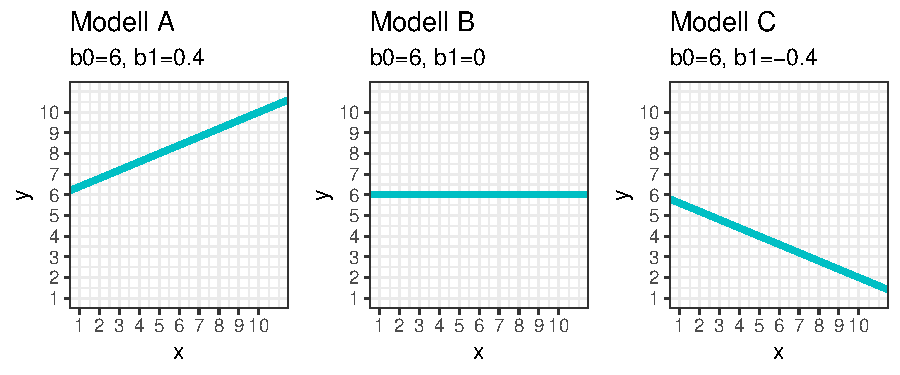
\includegraphics[width=1\linewidth]{04-h0_files/figure-latex/unnamed-chunk-2-1} 

}

\caption{**CAPTION THIS FIGURE!!**}\label{fig:unnamed-chunk-2}
\end{figure}

\textbf{Oppgave}

\begin{enumerate}
\def\labelenumi{\alph{enumi}.}
\tightlist
\item
  La oss si at vi hatt med et målt et individ sin \textbf{X} og \textbf{Y} (du kan bytte ut X og Y med hvilken som helst variabel (f.eks. høyde, vekt), hvis du vil). Individet sitt mål på X er 8. Hvis du bruker modell A, hva vil du forvente at denne personen har på \emph{Y}?
\end{enumerate}

.

I figuren ser du tre modeller som har forskjellige b0, men samme b1. b0 er verdien på Y når X er 0.

\begin{figure}

{\centering 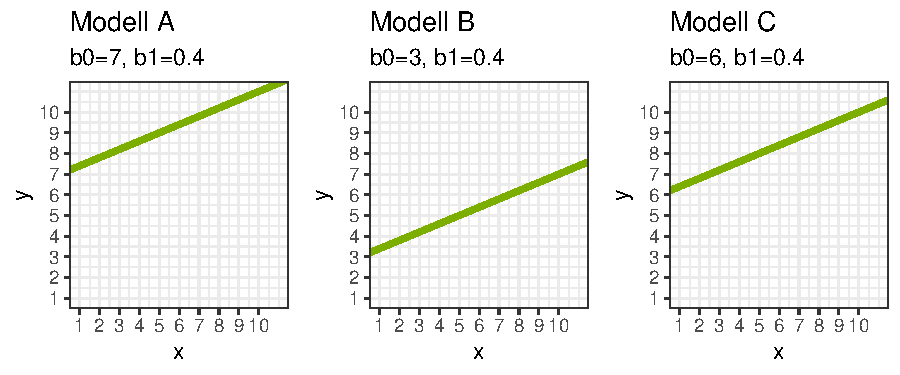
\includegraphics[width=1\linewidth]{04-h0_files/figure-latex/unnamed-chunk-3-1} 

}

\caption{**CAPTION THIS FIGURE!!**}\label{fig:unnamed-chunk-3}
\end{figure}

\textbf{Oppgave}

\begin{enumerate}
\def\labelenumi{\alph{enumi}.}
\tightlist
\item
  La oss si at vi hatt med et målt et individ sin \textbf{X} og \textbf{Y} (du kan bytte ut X og Y med hvilken som helst variabel (f.eks. høyde, vekt), hvis du vil). Individet sitt mål på X er 3. Hvis du bruker modell B, hva vil du forvente at denne personen har på \emph{Y}?
\end{enumerate}

.

\begin{quote}
\begin{quote}
Håper du har fått en liten innføring i ulike modeller.
\end{quote}
\end{quote}

\hypertarget{modellbygging-med-null-hypothesis-significance-testing-nhst}{%
\section{Modellbygging med `Null-Hypothesis Significance Testing (NHST)'}\label{modellbygging-med-null-hypothesis-significance-testing-nhst}}

Nå som du har en fått en innføring i hvordan du kan bygge modeller er det på tide at vi begynner å spesifisere hvilke modeller vi skal bygge. Som du sikkert er kjent med jobber forskere innenfor et paradigme som kalles for \textbf{Null-Hypothesis Significance Testing (NHST)}. Dette går ut på at forskeren fremstiller to hypoteser:

\begin{enumerate}
\def\labelenumi{\arabic{enumi}.}
\tightlist
\item
  \textbf{H0}: En null-hypotese som sier at det ikke er noen effekt (f.eks. ingen forskjeller mellom grupper, ingen sammenheng mellom variablene)
\item
  \textbf{H1}: En alternativ/eksperimentell hypotese som sier at det er en effekt (f.eks. det er en forskjell mellom gruppene)
\end{enumerate}

For å teste disse hypotesene må forskeren bygge to modeller:
- en modell for null-hypotesen (vi kaller denne for \textbf{null-modellen})
- en alternativ-modell som sier det at det er en relasjon eller forskjeller mellom grupper.

Vi regner ut hvor mye error det er i hver av disse modellene for å se hvilke av disse modellene det er klokt å benytte. Husk at målet er å benytte modeller som er gode og som har lite error. Hvis null-modellen er god nok, så er det ikke noe poeng å bruke den alternative modellen. Men hvis den alternative modellen er mye bedre enn null-modellen, da bør benytte denne.

Statistikken hjelper oss med å ta en beslutning om hvilke av disse modellene vi skal bruke. Forskeren gjennomfører deretter en \textbf{statistisk test} som representerer den alternative hypotesen. Utfallet av testen er en \textbf{verdi}, for eksempel en \emph{z-verdi}, \emph{t-verdi} eller \emph{f-verdi}, som vi kan bruke til å regne ut sannsynligheten (\emph{p}-verdi)for, gitt at null-hypotesen er sann. Forskjellige tester opererer med forskjellige navn på verdiene sine (sorry, men det er bare slik det er).

\begin{quote}
\begin{quote}
Vi kommer til å ha fokus på å bygge modeller her
\end{quote}
\end{quote}

\begin{figure}

{\centering 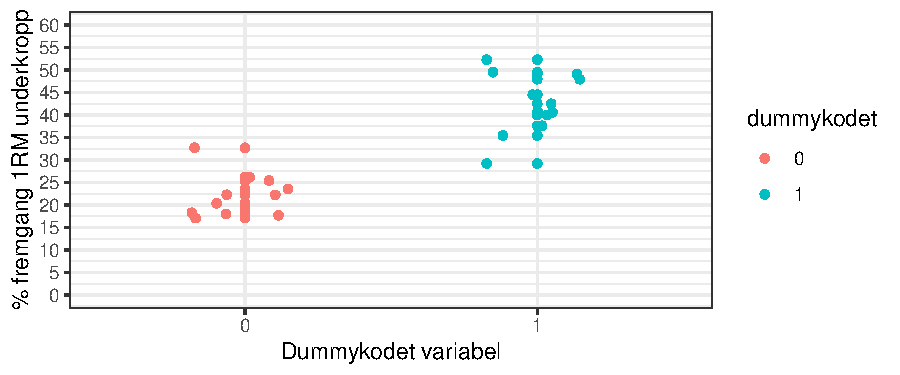
\includegraphics[width=1\linewidth]{04-h0_files/figure-latex/unnamed-chunk-4-1} 

}

\caption{**CAPTION THIS FIGURE!!**}\label{fig:unnamed-chunk-4}
\end{figure}

\hypertarget{null-modellen-null-hypotesen}{%
\section{Null-modellen (null-hypotesen)}\label{null-modellen-null-hypotesen}}

I vår studie ønsker vi å teste om det er forskjeller mellom de to gruppene som har blitt disponert for ulikt treningsopplegg (3 versus 1 sett). Husk at vi har laget en variabel hvor vi har kodet disse som 0 og 1; 0 hvis de trente med ett sett og 1 hvis de trente tre sett. Null-hypotesen er at det ikke er noen forskjeller mellom gruppene. I så fall er gjennomsnittet 1 RM fremgang av alle deltakerne kanskje en god modell. Dette er modellen som representerer null-hypotesen. Med andre ord vår null-modell

\[
Y_i = (b_0) + error
\]
\[
fremgang.1RM = (mean) + error
\]
Det er ofte enklere å se denne modellen i tabellform, slik som dere ser under.

\label{tab:unnamed-chunk-6}Null-modellen (mean)

individ

gruppe

rm

modell.mean

error

1

tre.sett

40.467

32.162

8.305

2

tre.sett

49.072

32.162

16.910

3

tre.sett

47.941

32.162

15.779

4

tre.sett

44.514

32.162

12.352

5

tre.sett

52.288

32.162

20.125

6

tre.sett

40.018

32.162

7.855

7

tre.sett

49.484

32.162

17.322

8

tre.sett

29.210

32.162

-2.952

9

tre.sett

40.593

32.162

8.431

10

tre.sett

37.587

32.162

5.424

11

tre.sett

35.427

32.162

3.264

12

tre.sett

42.494

32.162

10.331

13

ett.sett

17.706

32.162

-14.457

14

ett.sett

17.072

32.162

-15.091

15

ett.sett

18.268

32.162

-13.894

16

ett.sett

25.426

32.162

-6.736

17

ett.sett

32.703

32.162

0.541

18

ett.sett

19.102

32.162

-13.060

19

ett.sett

22.238

32.162

-9.924

20

ett.sett

22.271

32.162

-9.891

21

ett.sett

26.179

32.162

-5.983

22

ett.sett

20.349

32.162

-11.814

23

ett.sett

23.528

32.162

-8.635

24

ett.sett

17.960

32.162

-14.203

\textbf{Oppgave}

La oss prøve hvordan denne modellen virker. For individ 1 målte vi en fremgang i 1RM underkropp på \textbf{40.467}, men modellen vår sa \textbf{32.162}. Så modellen bommet med 8.305, dvs. en error på \textbf{8.305}.
\[
fremgang.1RM = (mean) + error
\]
\[
40.467 = 32.162 + 8.305
\]

\begin{enumerate}
\def\labelenumi{\alph{enumi}.}
\tightlist
\item
  Prøv modellen du også: For individ nr. 8, sier modellen at individet hadde en skår på , men denne personen hadde faktisk en skår på . Modellen bommet derfor med .
\end{enumerate}

\begin{quote}
\begin{quote}
Vi kan fortsette slik for alle deltakerne vi har hatt med i studien. Husk at vi ikke er interessert i hvir mye bommer for hvert enkelt individ, men for alle indivene.
\end{quote}
\end{quote}

\begin{enumerate}
\def\labelenumi{\alph{enumi}.}
\setcounter{enumi}{1}
\tightlist
\item
  Hva får du hvis du summerer all erroren for alle indidene? null 0 3 -3.
\end{enumerate}

\begin{quote}
\begin{quote}
tenk over hvorfor du får dette svaret før du leser videre.
\end{quote}
\end{quote}

\begin{quote}
\begin{quote}
Som du så i forrige oppgave blir det feil å summere alle erroren, vi kan løse dette effektivt ved ved å regne \textbf{Sum of Squared Error}. Det vi gjør er å gange error med seg selv (error\^{}2) før vi summerer alt dette sammen.
\end{quote}
\end{quote}

\begin{enumerate}
\def\labelenumi{\alph{enumi}.}
\setcounter{enumi}{2}
\tightlist
\item
  Hvis vi regner ut \textbf{Sum of Squared Error} for null-modellen fpr vi:
\end{enumerate}

\begin{quote}
\begin{quote}
Dette tallet er viktig! Dette er null-hypotesen vår! Hvis det ikke er noen forskjell mellom de to treningsgruppene våre er det like greit å bruke denne null-modellen. Men hvis vi finner ut at modellen vår blir bedre (dvs. reduserer Sum of Squared Error) ved å legge til en prediktorvariabel som består er av gruppevariabelen vår, da bør vi gjøre dette.
\end{quote}
\end{quote}

Før du går videre er det greit å visualisere hvordan null-hypotesen ser ut rent visuelt. Den prikkete streken i figuren under representerer modellen vår som er mean. Som du ser, så gjør den ingen justeringer for de ulike individene. Erroren er avstanden fra den linjen og opp til hvert datapunkt. Så hvis vi får til å bygge en bedre modell så vil denne avstanden reduseres for alle individene.

\begin{figure}

{\centering 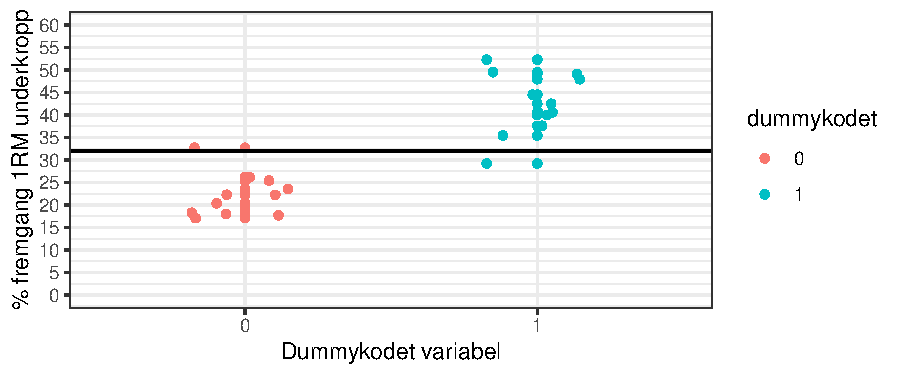
\includegraphics[width=1\linewidth]{04-h0_files/figure-latex/unnamed-chunk-8-1} 

}

\caption{**CAPTION THIS FIGURE!!**}\label{fig:unnamed-chunk-8}
\end{figure}

\hypertarget{alternativ-modell-alternativ-hypotese}{%
\section{Alternativ modell (alternativ hypotese)}\label{alternativ-modell-alternativ-hypotese}}

I forrige avsnitt sa vi at \textbf{null-hypotesen (H0)} reresenterer en en modell som gir samme prediksjon for alle deltakerne som var med i studien uavhengig av hvilken treningsgruppe de tilhører. Vi kalte denne for null-modellen. Vi regnet oss også frem til at denne modellen ga oss en Som of Squared error på 3243.784.

Spørsmålet vi skal stille i dette nå er om vi kan redusere error fra denne ved å benytte en mer kompleks modell som benytter (vår dummykodede kategoriske variabel) som prediktorvariabel:
\[
Y_i = (b_0 + b_1X_i) + error
\]
Prediktorvariabelen b1 er en gruppevariabelen vår som vi dummykodet med tallene 0 og 1.

\[
Fremgang.1RM_i = b_0 + b_1(Gruppe) + error_i
\]
For å holde dette på et overordnet nivå, så vil jeg gi dere de estimerte verdiene for b0 og b1. Målet er å vise dere hvordan denne modellen fungerer. Senere skal gå gjennom hvordan vi regner ut disse verdiene. Trykk her hvis du ønsker å finne ut hvoran du regner ut disse verdiene med en gang.

\[
Fremgang.1RM_i = b_0(21.90) + b_1(20.52*Gruppe) + error_i
\]
Modellen sier at vår b0 er 21.90. Dette er den forventede verdien på Y (Fremgang.1RM) når prediktorvariabelen er 0. Modellen sier også at b1 er 20.52. Med andre ord den forventede økning i Y for en enhets økning i X (også kalt stigningstallet). Husk at vi lagde en gruppe-variabel der vi kodet de to gruppene våre med 0 og 1. Så hvis et individ tilhørte gruppe 0, blir vår prediksjon:

\[
Fremgang.1RM_i = 21.90 + b_1(20.52*0) + error_i
\]
Fordi 0*20.52 = 0, blir stående igjen med b0. Vår prediksjon av et individ som tilhører gruppe 0 blir

\[
Fremgang.1RM_i = 21.90 + 0 + error_i
\]
\[
Fremgang.1RM_i = 21.90 + error_i
\]
Hvis individet derimot tilhører 1 predikerer modellen at individet sin skår blir 42.48.

\[
Fremgang.1RM_i = 21.90 + b1(20.52*1) + error_i
\]
\[
Fremgang.1RM_i = 42.48 + error_i
\]
Visualisert fremstilt blir modellen vår seendes slik ut:

\begin{Shaded}
\begin{Highlighting}[]
\FunctionTok{ggplot}\NormalTok{(dat, }\FunctionTok{aes}\NormalTok{(dummykodet, rm, }\AttributeTok{color=}\NormalTok{dummykodet)) }\SpecialCharTok{+}
  \FunctionTok{geom\_point}\NormalTok{()}\SpecialCharTok{+}
  \FunctionTok{scale\_y\_continuous}\NormalTok{(}\AttributeTok{breaks =} \FunctionTok{seq}\NormalTok{(}\DecValTok{0}\NormalTok{, }\DecValTok{60}\NormalTok{, }\DecValTok{5}\NormalTok{)) }\SpecialCharTok{+}
  \FunctionTok{coord\_cartesian}\NormalTok{(}\AttributeTok{ylim =} \FunctionTok{c}\NormalTok{(}\DecValTok{0}\NormalTok{, }\DecValTok{60}\NormalTok{)) }\SpecialCharTok{+}
  \FunctionTok{geom\_jitter}\NormalTok{(}\AttributeTok{width =} \FloatTok{0.2}\NormalTok{) }\SpecialCharTok{+} 
  \FunctionTok{stat\_summary}\NormalTok{(}\AttributeTok{geom =} \StringTok{"line"}\NormalTok{, }\AttributeTok{fun =}\NormalTok{ mean, }\AttributeTok{group =} \DecValTok{1}\NormalTok{, }\AttributeTok{color=}\StringTok{"black"}\NormalTok{, }\AttributeTok{linetype=}\StringTok{"dotted"}\NormalTok{, }\AttributeTok{size=}\FloatTok{1.2}\NormalTok{) }\SpecialCharTok{+}
  \FunctionTok{labs}\NormalTok{(}\AttributeTok{y=}\StringTok{"\% fremgang 1RM underkropp"}\NormalTok{, }\AttributeTok{x=}\StringTok{"Dummykodet variabel"}\NormalTok{) }\SpecialCharTok{+}
  \FunctionTok{theme\_bw}\NormalTok{()}
\end{Highlighting}
\end{Shaded}

\begin{figure}

{\centering 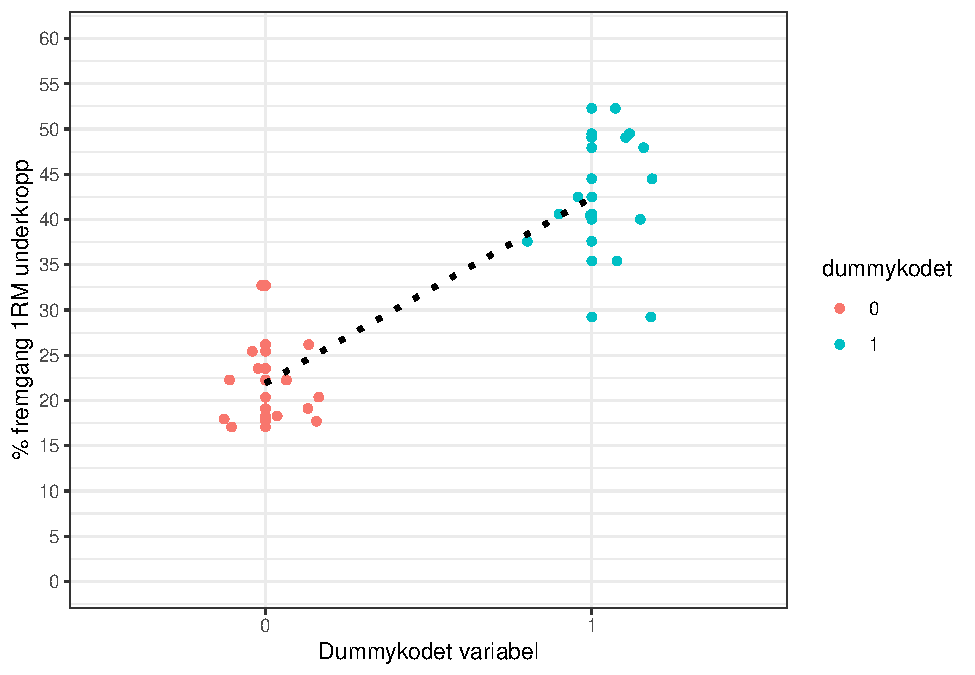
\includegraphics[width=1\linewidth]{04-h0_files/figure-latex/unnamed-chunk-9-1} 

}

\caption{**CAPTION THIS FIGURE!!**}\label{fig:unnamed-chunk-9}
\end{figure}

\textbf{Oppgave}
Tabellen under viser 6 individer som tilhørte treningsgruppe. Du ser deres faktiske fremgang i 1RM kolonnen. La oss bruke det vi har lært til å predikere disse personene sin fremgang. Vi bruker samme modell som over

\[
Fremgang.1RM_i = b_0(21.90) + b_1(20.52*Gruppe) + error_i
\]
a. Hva predikerer modellen at individ nummer 3 hadde i skår? (to desimaler)

b, Hva hadde individ nr i skår?

\begin{enumerate}
\def\labelenumi{\alph{enumi}.}
\setcounter{enumi}{2}
\tightlist
\item
  hvor mye error blir det?
\end{enumerate}

\begin{enumerate}
\def\labelenumi{\alph{enumi}.}
\setcounter{enumi}{3}
\tightlist
\item
  i Squared Error blir denne erroren?
\end{enumerate}

\begin{enumerate}
\def\labelenumi{\alph{enumi}.}
\setcounter{enumi}{4}
\item
  nå som du har jobbet med denne modellen, så lurer jeg på om det er noe kjent med disse verdiene i modellen. Gå tilbake til {[}link{]} hvis du trenger et hint.
\item
  bo er (norskt ord) for gruppen som er kodet med 0.
\item
  b1 er (norsk ord) mellom gruppen som er kodet med 0 og gruppen som er kodet med 1.
\item
  b0 + b1 er (norsk ord) for gruppen som er kodet med 1.
\end{enumerate}

\begin{table}

\caption{\label{tab:unnamed-chunk-11}Dummy koding}
\centering
\begin{tabular}[t]{r|l|r|r}
\hline
individ & gruppe & rm & dummykodet\\
\hline
1 & tre.sett & 40.467 & 1\\
\hline
2 & tre.sett & 49.072 & 1\\
\hline
3 & tre.sett & 47.941 & 1\\
\hline
4 & tre.sett & 44.514 & 1\\
\hline
5 & tre.sett & 52.288 & 1\\
\hline
6 & tre.sett & 40.018 & 1\\
\hline
\end{tabular}
\end{table}

I forrige oppgave regnet du ut error for ett enkelt individ. Men vi er interessert i den totale erroren for modellen. Formelen for denne er:

total error in den alternative modellen:

SS\_R = \(\sum_{n=1}^N (observert_i - modell_i)^2\)

Med andre ord er det kvadraten av den faktiske observasjonen - hva modellen sa. Bruk formelen til å regne ut dette. (to desimaler

\hypertarget{anova-tabell-variansanalyse}{%
\section{ANOVA-tabell (variansanalyse)}\label{anova-tabell-variansanalyse}}

Nå har vi bygget to modeller og regnet ut hvor mye error det er hver av disse modellene - \textbf{null-modell} og \textbf{den alternative modellen}. Vår neste oppgave er å \textbf{sammenligne disse modellene}. For å gjøre det helt tydelig, så skal vi steste om modellen til høyre er bedre enn modellen til venstre. Når vi sier bedre, så mener vi at den har mindre error i seg.

\begin{figure}

{\centering 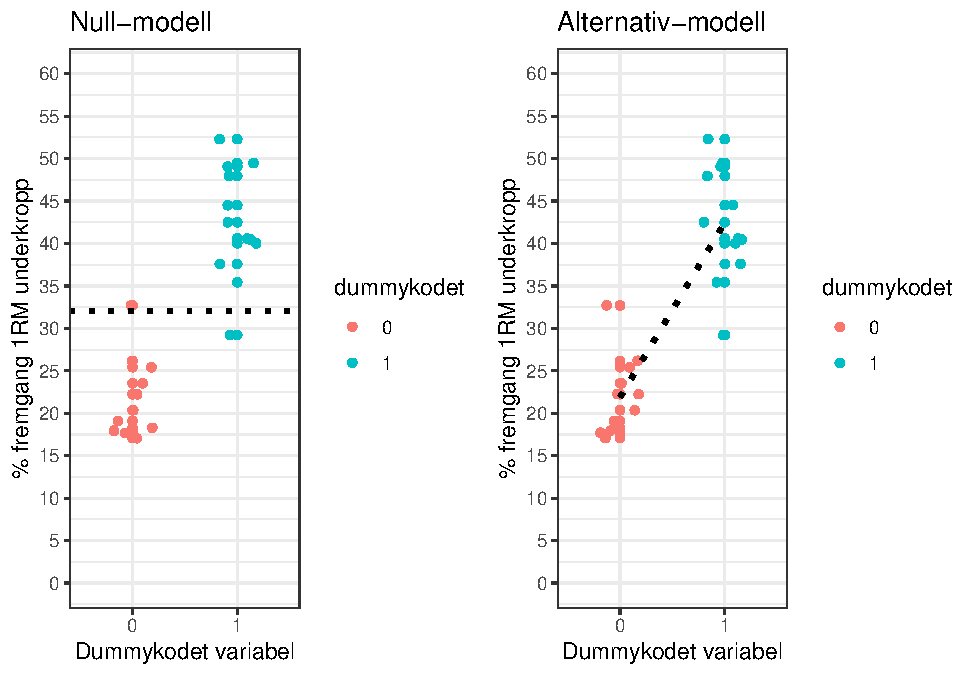
\includegraphics[width=1\linewidth]{04-h0_files/figure-latex/unnamed-chunk-12-1} 

}

\caption{**CAPTION THIS FIGURE!!**}\label{fig:unnamed-chunk-12}
\end{figure}

For å sammenligne disse modellene er det vanlig å bruke en ANOVA-tabell. Dette er en ganske vanlig tabell som dere kommer til å se mange ganger, så det er bare å bli vant til å se disse. Dere har allerede regnet ut all nødvendig informasjon for å lage en ANOVA-tabell, så dere kan lage den selv.

\textbf{ANOVA-tabell}

\begin{longtable}[]{@{}llllll@{}}
\toprule
Modell & SS & \emph{df} & MS & \emph{F} & R2\tabularnewline
\midrule
\endhead
The model sum of squares (SSM) & & & & &\tabularnewline
The residual sum of squares (SSR) & & & & &\tabularnewline
The total sum of squares (SST) & & & & &\tabularnewline
\bottomrule
\end{longtable}

\textbf{Oppgave}

\begin{enumerate}
\def\labelenumi{\alph{enumi}.}
\tightlist
\item
  Hva var sum of squared error for null-modellen?
\end{enumerate}

\begin{quote}
\begin{quote}
(Sett dette inn i total sum of squares (SST)
\end{quote}
\end{quote}

\begin{enumerate}
\def\labelenumi{\alph{enumi}.}
\setcounter{enumi}{1}
\tightlist
\item
  Hva var sum of squared error for den alternative modellen?
\end{enumerate}

\begin{quote}
\begin{quote}
(Sett dette inn i residual sum of squares (SSR). Dette er error som er igjen etter at man har brukt den alternative-modellen. Men \textgreater\textgreater andre ord. Man kalles dette residuals.
\end{quote}
\end{quote}

\begin{enumerate}
\def\labelenumi{\alph{enumi}.}
\setcounter{enumi}{2}
\tightlist
\item
  Hvor mye sum of squared error er redusert ved å bruke den alternative modellen i forhold null-modellen?
\end{enumerate}

\begin{quote}
\begin{quote}
Dette kalles The model sum of squares (SSM) eller regression i statistiske programmer.
\end{quote}
\end{quote}

Før vi går videre er det greit å visualisere erroren som er igjen med de to modellene, pluss hvor mye error som er redusert ved å bruke den alternative modellen istf. å bruke null-modellen. I figuren under ser du de tre modellene. SST representerer den totale erroren (dvs. erroren vi fikk ved å bruke null-modellen); SSR representerer hvor mye error som er igjen etter at vi brukte den alternative modellen. SSM er hvor mye error som modellen vår klarte å forklare. Vil du si at den alternative modellen vår er god?

\begin{quote}
\begin{quote}
Hint. Hvis du summerer SSM og SSR får du SST
\end{quote}
\end{quote}

Sammenlign dette med modellen til høyre. Her har vi en modell som er dårlig fordi SSM er lav og SSR er høy.

\begin{quote}
\begin{quote}
For sikkerhets skyld. Modellen til høyre ble bare brukt som et eksempel for at du skal forstå at vi kan vurdere hvor god modellen vår er.
\end{quote}
\end{quote}

\begin{figure}

{\centering 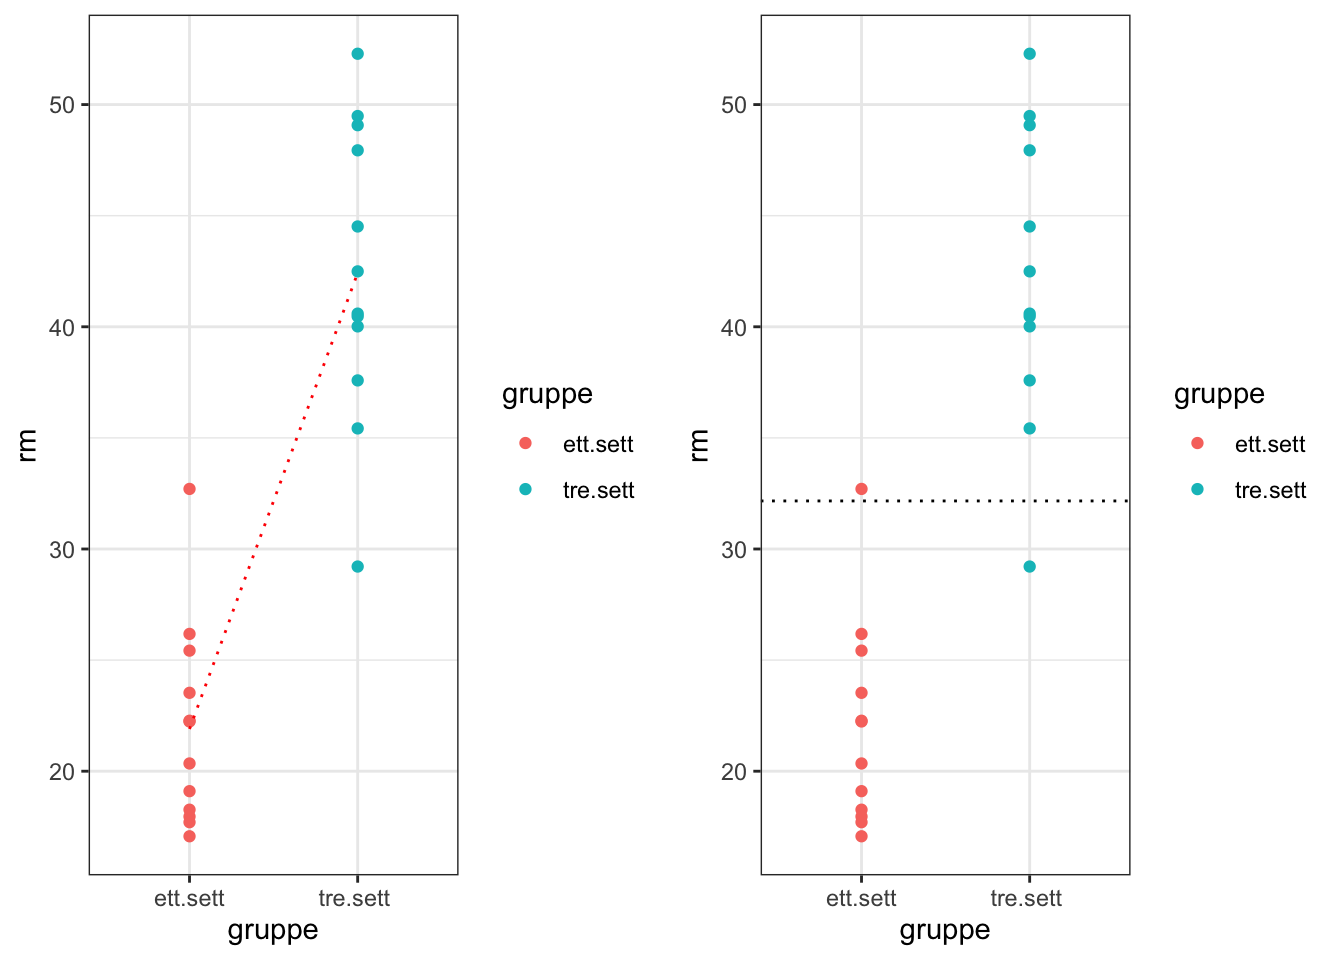
\includegraphics[width=1\linewidth]{04-h0_files/figure-latex/unnamed-chunk-13-1} 

}

\caption{**CAPTION THIS FIGURE!!**}\label{fig:unnamed-chunk-13}
\end{figure}

\begin{enumerate}
\def\labelenumi{\alph{enumi}.}
\setcounter{enumi}{4}
\tightlist
\item
  Basert på det du ser i figuren over til venstre, vil du si at vår alternative modell er god?
\end{enumerate}

ja nei.

\begin{enumerate}
\def\labelenumi{\alph{enumi}.}
\setcounter{enumi}{3}
\tightlist
\item
  Hva er (SST) - (SSR)?
\end{enumerate}

\begin{enumerate}
\def\labelenumi{\alph{enumi}.}
\setcounter{enumi}{4}
\tightlist
\item
  Hva er (SSR) + (SSM)?
\end{enumerate}

Vi kan regne ut hvor mange \% modellen vår har redusert error med, og dette er gange nyttig. Dette får dere vite når dere kjører en test i Jamovi eller R, men vi kan også regne det for hånd. Verdien fi vår kalles \(R^2\).

\[
R^2 = \frac{(SS_T - SS_R)}{SS_T} * 100
\]

\begin{enumerate}
\def\labelenumi{\alph{enumi}.}
\setcounter{enumi}{4}
\tightlist
\item
  Hvilken verdi får du hvis du regner (SSM/ (SST)) * 100?
\end{enumerate}

(uten \%-tegnet)

\begin{quote}
\begin{quote}
Det er dessverre mange forskjellige navn på denne verdien. Du vil se at folk bruker PRE, \(n^2\). Vit at de mener det samme.
\end{quote}
\end{quote}

Det kan høres ut som at en errorreduksjon på 78 \% er mye, og det vil vi absolutt påstå at det er! Kan vi da konkludere at den alternative modellen er bedre enn null-modellen? - det ser jo ut til at dette er mye.

\hypertarget{teste-null-hypotesen-med-f}{%
\section{teste null-hypotesen med F}\label{teste-null-hypotesen-med-f}}

For å teste om en SSM eller en errorreduksjon på 78 \% er mye eller lite skal vi bruke en F-test og en F-fordeling. En F-fordeling ser veldig lik ut som en z og t-fordeling og fungerer på samme måte: Vi regner ut en F-verdi, og spør fra sannsynligheten er for å oppnå en slik verdi gitt at null-hypotesen er sann. Null-hypotesen i en F-test er at den alternative modellen ikke forklarer noe varians. Med andre ord at \(R^2\) = 0. For å teste dette må vi regne ut en F-verdi:

\[
F = \frac{(SS_M / df_M)}{SS_R / df_R}
\]
Vi har allerede regne ut, så vi kan plotte disse inn.

\[
F = \frac{(<input class='solveme nospaces' size='6' data-answer='["2527.5"]'/> / df_M)}{716.2875 / df_R}
\]
Men hva er de respektivene frihetsgradene som er i nevneren og telleren? Å forstå dette vil gi en god forståelse for hva F-verdien er. Vi fokuserer på telleren først. Modellen reduserte Sum of Squared error med 2527.5, som i grunn er mye. Men vi kunne bygget en superkompleks og lagt til haugevis av ekstra parametere. Dette kunne vi gjort ved å f.eks sammenlignet enda flere grupper. Vi har ikke lært hvordan vi gjør dette enda, men vi kan fint gjøre det. Og vi skal vise hvordan senere. Vi kunne derfor i prinsippet ha gått fra:

\[
Y_i = b_0
\]
til:
\[
Y_i  = b_0 + b_1X_i + b_2X_i + b_3X_i + b_4X_i + b_5X_i
\]
I så fall ville vi garantert ha fått en stor Sum of squared error fordi et parameter alltid vil redusere error noe, aldri øke det. Så det vi skal gjøre i telleren i formelen er å dele på SSm / på antall parametere vi har brukt utover det null-modellen har brukt. Null-modellen hadde kun ett parameter, mens den altenative modellen hadde 2, så df blir 1. Poenget som jeg vil at dere skal huske på er at. Dette er variansen. Poenget er en SSm er mer imponerende om vi har brukt få ekstra parametere.

Husk at når vi trekker to eller flere utvalg fra en populasjon, så vil disse utvalgene nesten alltid være forskjellige fra hverandre.

Vi kunne bruke samme prinsipp for t-fordelingen. Null-hypotesen var disse tilfellene var at disse

Felles for disse fordelingene er at de baserer seg på gjennomsnittet mellom utvalg. V

Da vi brukte en \emph{z}-fordeling sa vi at 95 \% av utvalgene vi trekker fra en populasjon med et gjennomsnitt på 0 og et standardavvik på 1, ville falle mellom en z-verdi på -1.96 og 1.96, gitt at de ble trukket fra denne populasjonen. Hvis vi plutselig observerte en z-skår for vårt utvalg som høyere enn 1.96 eller lavere enn -1.96, sa vi at vi hadde et signifikant funn og at utvalgene dermed ikke kommer fra samme populasjon. Vi brukte en t-fordeling på lignende måte.

Men hvis vi brukte en z-fordeling, så sa vi at 95 \% av utvalgene vi trekker fra en slik fordeling vil falle mellom en z-verdi mellom -1.96 og 1.96. Vi kan bruke en t-fordeling til å si noe lignende. Felles for z-fordelingen og t-fordelingen er de går på sample means. En f-fordeling baserer seg ikke på means, men på reduksjon i sum of squared errors. Null-hypotesen er at det ikke modellen vår reduserer noe error i det hele tatt. Men fordi forskjellige utvalg gir forskjellige, må vi forvente at det er noen fordelinger under null

Vi har allerede jobbet med to fordelinger, en z-fordeling, t-fordeling. Det vi skal jobbe med nå er en F-fordeling. En F-fordeling er nesten likt som en z-fordeling og en t-fordeling, men er litt forskjellig fra disse på den måten at en F-fordeling operer med forklart Sum of Squarered error ved modellen, mens en z-fordeling og t-fordeling operer med sample means. Med andre ord, istf. å si hva er sannsynlig for observere en t, gitt att, skal vi spørre hva er sannsynligheten for at det ikke noe explained varians. Gitt at null hypotesen er sann, dvs.. Selv om vi har explained variance i populasjonen, så vil det alltid være litt explained variance fra utvalg til utvalg. Dere husker kanskje. Så det vi må gjøre er å regne ut hvor mye hvor mye f-verdi, og så spørre oss, hva er sannsynligheten for å få en f-statistikk, så stor som denne, gitt at null hypotesen er sann. Explianed variansen av denne modellen er null.

For å finne ut av dette må vi regne ut en f-verdi. Formelen for dette er

\hypertarget{teste-null-hypotesen-med-t}{%
\section{teste null-hypotesen med t}\label{teste-null-hypotesen-med-t}}

Nå har vi kun lagt til ett ekstra parameter i forhold til null-modellen; vi gikk fra:

\[
Y_i = b_0
\]
til:

\[
Y_i = b_0 + b_1X_i
\]

Men tenk om vi hadde lagt til enda flere prediktorvariabler i modellen. Vi har ikke lært hvordan vi gjør dette enda, men vi kan fint gjøre det. Og vi skal vise hvordan senere. Vi kunne derfor i prinsippet ha gått fra:

\[
Y_i = b_0
\]
til:
\[
Y_i  = b_0 + b_1X_i + b_2X_i + b_3X_i + b_4X_i + b_5X_i
\]
I så fall ville vi garantert ha fått en stor errorreduksjon fordi noen av disse parameterne ville vært gode. Derfor regner vi gjennomsnittlig squared error, som vi kaller for \textbf{Mean Squared Error (MSE)}. Poenget med dette er at høy errorreduksjon med en alternativ modellen er mye mer imponerende hvis vi kun har med en prediktorvariabel enn om vi har med mange. Derfor regner vi \textbf{Mean SquaredM Model (MSE)}. MSE regnes ved å ta SSM / frihetsgrader (\emph{df}). Frihetsgradene vi bruker til dette er antatt ektra parametere vi har lagt til i modellen vår med referanse til null-modellen. Vi hadde 2 parametere i den alternative modellen og 1 i null-modellen, så 2-1.

\begin{enumerate}
\def\labelenumi{\alph{enumi}.}
\setcounter{enumi}{5}
\tightlist
\item
  Regn ut \textbf{Mean Squared Model (MSM)} og putt den inn i ANOVA-tabellen. \(MS_M=\frac{(SS_M)}{df}\). Legg samtidig antall frihetsgrader for MSE inn i ANOVA-tabellen over.
\end{enumerate}

Det neste vi skal gjøre er å regne er \textbf{Mean Squared (MSM)}

\begin{enumerate}
\def\labelenumi{\alph{enumi}.}
\setcounter{enumi}{6}
\item
  Det aller siste vi skal gjøre er å
\item
  I cellen under har jeg kjørt en ANOVA-test. Virker resultatene kjent. Skriv \emph{p}-verdien din inn i?
\end{enumerate}

Hvis dette ikke var forståelig foreslår jeg følgende tutorials:
- \url{https://www.youtube.com/watch?v=eSJAjlavPwU}
- \url{https://www.youtube.com/watch?v=0xWDulRHd9M}
- \url{https://www.youtube.com/watch?v=iAE4UeoVE9A}
- \url{https://www.youtube.com/watch?v=OK4Xns4zabs}

\begin{Shaded}
\begin{Highlighting}[]
\CommentTok{\#aov er en forkortolse for analysis of variance (ANOVA)}
\CommentTok{\#dette er funksjon som kommer mer R.}
\FunctionTok{summary}\NormalTok{(}\FunctionTok{aov}\NormalTok{(rm }\SpecialCharTok{\textasciitilde{}}\NormalTok{ dummykodet, dat))}
\end{Highlighting}
\end{Shaded}

\begin{verbatim}
##             Df Sum Sq Mean Sq F value   Pr(>F)    
## dummykodet   1 2527.5  2527.5   77.63 1.15e-08 ***
## Residuals   22  716.3    32.6                     
## ---
## Signif. codes:  0 '***' 0.001 '**' 0.01 '*' 0.05 '.' 0.1 ' ' 1
\end{verbatim}

\begin{figure}

{\centering 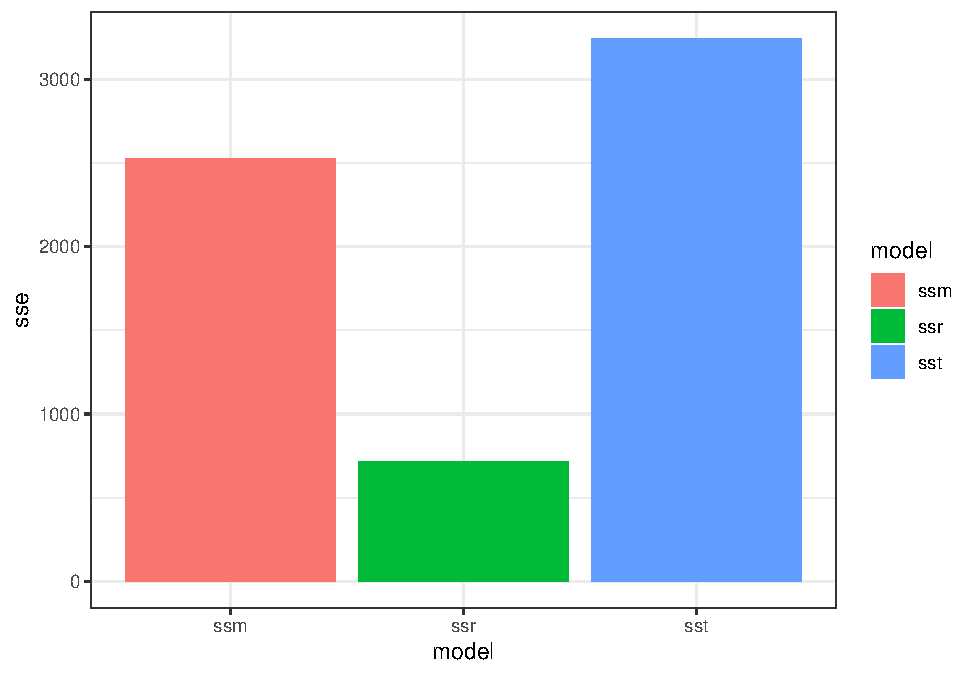
\includegraphics[width=1\linewidth]{04-h0_files/figure-latex/unnamed-chunk-16-1} 

}

\caption{**CAPTION THIS FIGURE!!**}\label{fig:unnamed-chunk-16}
\end{figure}

\hypertarget{hvordan-finne-linjen-i-modellen}{%
\section{Hvordan finne linjen i modellen?}\label{hvordan-finne-linjen-i-modellen}}

Nå som vi er kjent med hvordan vi kan bygge og teste statistiske modeller, er det på tide å vise hvordan vi finner regresjonslinjen som vi skal bruke. Mer presist, hvilke verdier skal vi ha for \emph{b}0 og \emph{b}1 som beskriver denne linjen? Hittil har dere fått disse verdiene av meg, men det vi skal lære nå er hvordan vi kan regne ut disse verdiene for hånd. En viktig sannhet om denne linjen er at regresjonslinjen (les modellen) er plassert slik at den reduserer Sum of Squared Error mest mulig. Med andre ord, verdiene på \emph{b}0 og \emph{b}1 (som beskriver denne linjen) er slik at det er umulig å redusere error mer. Spørsmålet er hvordan vi finner verdiene på \emph{b}0 og \emph{b}1 som beskriver denne linjen. En tilnærming kan være å gjette seg fram til hva \(b_0\) og \(b_1\) skal være. Vi kan teste ut ulike verdier for b0 og b1, og evaluere hvor mye sum of Squared Error disse gir. I figuren under har jeg prøvd tre ulike modeller, og regner ut hvor mye sum of squared error disse gir.

\begin{figure}

{\centering 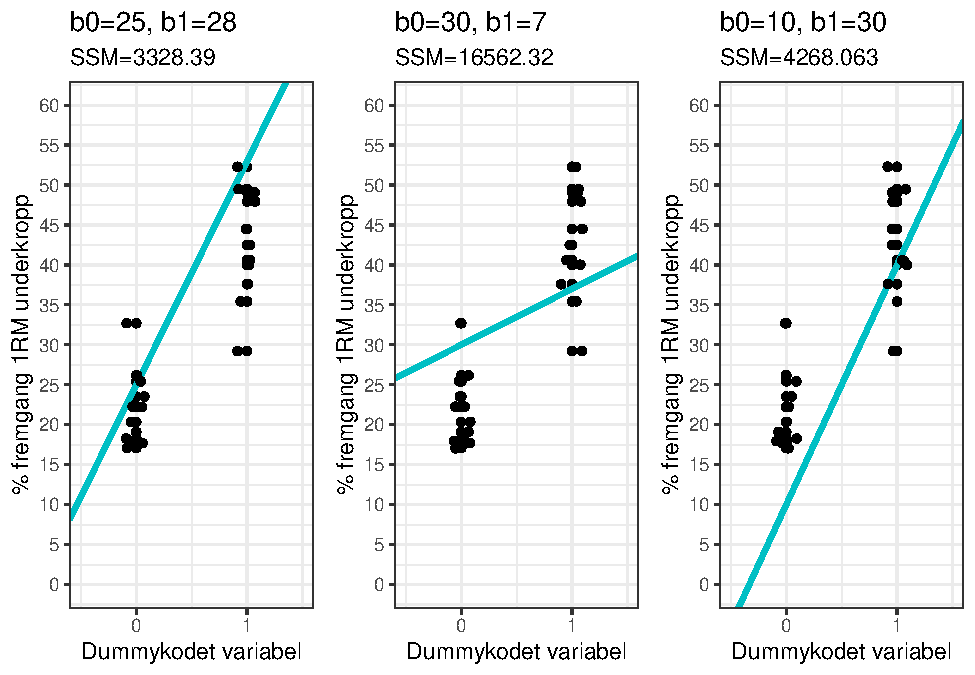
\includegraphics[width=1\linewidth]{04-h0_files/figure-latex/unnamed-chunk-17-1} 

}

\caption{**CAPTION THIS FIGURE!!**}\label{fig:unnamed-chunk-17}
\end{figure}

\textbf{Oppgave}
a) Hvilken av modellene over gir mest sum of squared error? (SSModel)

b0=30 b1=7 b0=25 b1=28 b0=10 b1=30

Vi kan holde på slik med slik prøving-og-feiling til vi faktisk finner linjen som reduserer error mest. Det er bare å teste nok verdier. \textbf{Minste kvadraters metode} garanterer oss å alltid gi oss er svar. Jeg har laget en video til dere som viser vi kan prøve-og-feile til vi kommer frem til en løsning (se denne):

Det er en mer effektiv måte å løse dette problemet på. For å finne \textbf{b1} kan vi bruke følgende formel:

\[ b_1 = \frac{SCP}{SS_x} \]
Her var det et nytt begrep, \textbf{SCP}. SCP står for sum of cross-product deviations. Det brukes til å finne relasjonen mellom to variabler, og er grunnlaget for en rekke utregninger i statistikken, så det kan være lurt å lære seg. SCP finner ut av om en person som er over eller under gjennomsnittet på en variabel, også er over eller under gjennomsnittet på den andre variabelen.

\[ b_1 = \frac{SCP = \sum_{n=1}^N (x_i - \bar{x})(y_i - \bar{y})}{SS_x} \]
\(\bar{x}\) er gjennomsnittet på x-variabelen (gruppe), mens \(\bar{y}\) er gjennomsnittet for y-variabelen (1RM). I tabellen under ser du hvordan vi regner dette. Kolonnen CrossProduct er \((x_i - \bar{x})(y_i - \bar{y})\).

\begin{table}

\caption{\label{tab:unnamed-chunk-18}Utregning av Sum of Cross Product (SCP)}
\centering
\begin{tabular}[t]{rrrrrrrr}
\toprule
individ & gruppe & gj.snitt.x & error.x & rm & gj.snitt.y & error.y & CrossProduct\\
\midrule
1 & 1 & 0.5 & 0.5 & 40.46704 & 32.16231 & 8.3047301 & 4.1523651\\
2 & 1 & 0.5 & 0.5 & 49.07223 & 32.16231 & 16.9099106 & 8.4549553\\
3 & 1 & 0.5 & 0.5 & 47.94131 & 32.16231 & 15.7789994 & 7.8894997\\
4 & 1 & 0.5 & 0.5 & 44.51389 & 32.16231 & 12.3515740 & 6.1757870\\
5 & 1 & 0.5 & 0.5 & 52.28750 & 32.16231 & 20.1251864 & 10.0625932\\
\addlinespace
6 & 1 & 0.5 & 0.5 & 40.01750 & 32.16231 & 7.8551872 & 3.9275936\\
7 & 1 & 0.5 & 0.5 & 49.48425 & 32.16231 & 17.3219362 & 8.6609681\\
8 & 1 & 0.5 & 0.5 & 29.21048 & 32.16231 & -2.9518368 & -1.4759184\\
9 & 1 & 0.5 & 0.5 & 40.59293 & 32.16231 & 8.4306117 & 4.2153059\\
10 & 1 & 0.5 & 0.5 & 37.58676 & 32.16231 & 5.4244472 & 2.7122236\\
\addlinespace
11 & 1 & 0.5 & 0.5 & 35.42651 & 32.16231 & 3.2641906 & 1.6320953\\
12 & 1 & 0.5 & 0.5 & 42.49354 & 32.16231 & 10.3312265 & 5.1656133\\
13 & 0 & 0.5 & -0.5 & 17.70576 & 32.16231 & -14.4565510 & 7.2282755\\
14 & 0 & 0.5 & -0.5 & 17.07181 & 32.16231 & -15.0905068 & 7.5452534\\
15 & 0 & 0.5 & -0.5 & 18.26811 & 32.16231 & -13.8942055 & 6.9471027\\
\addlinespace
16 & 0 & 0.5 & -0.5 & 25.42594 & 32.16231 & -6.7363771 & 3.3681886\\
17 & 0 & 0.5 & -0.5 & 32.70313 & 32.16231 & 0.5408147 & -0.2704074\\
18 & 0 & 0.5 & -0.5 & 19.10226 & 32.16231 & -13.0600552 & 6.5300276\\
19 & 0 & 0.5 & -0.5 & 22.23827 & 32.16231 & -9.9240435 & 4.9620217\\
20 & 0 & 0.5 & -0.5 & 22.27148 & 32.16231 & -9.8908322 & 4.9454161\\
\addlinespace
21 & 0 & 0.5 & -0.5 & 26.17889 & 32.16231 & -5.9834246 & 2.9917123\\
22 & 0 & 0.5 & -0.5 & 20.34857 & 32.16231 & -11.8137453 & 5.9068726\\
23 & 0 & 0.5 & -0.5 & 23.52773 & 32.16231 & -8.6345853 & 4.3172926\\
24 & 0 & 0.5 & -0.5 & 17.95966 & 32.16231 & -14.2026514 & 7.1013257\\
\bottomrule
\end{tabular}
\end{table}

\[ b_1 = \frac{SCP = 20.52436}{SSx} \]
Nå som vi har regnet SCP er det bare å regne SSx (sum of squared error for prediktorvariabelen) er fordi man ønsker å ta høyde for hvor mye prediktorvariabelen avviker fra mean. Jeg har dessverre ikke noen supergod forklaring, og jeg synes heller ikke Field forklarer dette godt. Så jeg bare vet at jeg må gjøre det.

\[ b_1 = \frac{SCP = 20.52436}{6} \]
\[ b_1 = 20.52436 \]

Nå gjenstår det bare å finne \textbf{b\_0}. Denne er enkel å finne når vi først har funnet \textbf{b0}. Husk at modellen vår er en ligning, så ved enkelt finne \textbf{b0} ved omorganisere ligningen: trekker vi fra \(b_1X_i\) på hver side av likhetstegnet får vi \textbf{b0} alene:

\[
Y_i = (b_0 + b_1X_i)
\]

\[
Y_i - b_1X_i = (b_0)
\]

Men må ligningen med verdier. Og da bruker man gjennomsnittet for Y variabelen og gjennomsnittet for X variabelen.

\[
32.16231     - (20.52436*0.5) = (21.90013)
\]

\hypertarget{t-test}{%
\section{T-test}\label{t-test}}

En ANOVA modell tester om vår alternative modell er bedre enn null-modellen totalt sett. Det neste vi kan gjøre er å se på de enkelte \emph{b}-ene i modellen. Husk at b1 er et stigningstall som representer den forventede endringen i utfallet for en enhets endring i prediktoren. Det vil med andre ord si tallet jeg forventer at Y øker med hvis jeg går fra 0 til 1, 2 til 3 eller 3 til 4 (alle disse er en enhetsøkning). Hvis verdien på b1 er 0 vil det ikke være noen relasjon mellom disse variablene. Hvis den er mer enn 0 er det en positiv relasjon mellom disse x og y; Hvis den er negativ er det en negativ relasjon mellom disse variablene. Husk at b1 i vårt tilfellet representer forskjellene i gjennomsnitt mellom de to gruppene. Så når vi går fra en enhets økning, vil vi forvente en økning i Y.

in the outcome resulting from a unit change in the predictor; if it is zero it means that as the predictor
changes, the outcome does not change at all

Remember that the value of b represents the change
in the outcome resulting from a unit change in the predictor; if it is zero it means that as the predictor
changes, the outcome does not change at all. In other words, there is no relationship. In
keeping with the logic of NHST, which the Secret Philanthropic Society told you about , we have
a null hypothesis that there is no relationship, and an alternative hypothesis that there is. A value
of b equal to 0 is our null hypothesis, and a value different from 0 is our alternative hypothesis

\hypertarget{write-up}{%
\chapter{Write-up}\label{write-up}}

Det er en ganske standardiser måte å rapporte en statistisk test på. Først skriver du hva har testet. Husk at du bare har gitt statistikprogrammet noen tall og fått et resultat. Nå må du kommunisere til andre.

'Deltakerne i 1L-3U 3L-1U-gruppen hadde i gjennomsnitt mindre større en lavere \% fremgang 1RM, på underkroppsøvelser (M=,SD=), enn som {[}{]}. Denne forskjellen, {[}{]}, CI {[}{]}, var signifikant, \emph{t}({[}{]}) = {[}{]}, p = {[}{]}, d={[}{]}.

  \bibliography{book.bib,packages.bib}

\end{document}
